\begin{appendices}
  
\chapter{APDL Language Introduction}
\label{app:tf-getting-started}

The syntax of the APDL language is very simple, and the goal of this document is to
provide a small introduction to APDL.

\section*{Creating a project}

A project is always identified by a name through the \apdlinline{project_name}
key-value pair. We could also fragment the project into multiple files and
include them with the \apdlinline{@include} keyword. So, an empty project looks
like :

\begin{apdlcode}
project_name = "Example"

@include "apdl_component.apdl"
@include "other_file.apdl"
\end{apdlcode}

We also need to note that the comments aren't supported for the moment.

\section*{Defining a device}

A device is the key entity of an APDL project, and it is defined by using the
\apdlinline{@device} keyword with an identifier. The identifier has to be unique
and don't containing any special character. The full grammar of APDL is available
in appendix \ref{app:apdl_ebnf_diagramm}.

When we define a device, we have to specify an ``id'' and a ``framework'' :
\begin{apdlcode}
@device example {
  id = Uno
  framework = arduino
}
\end{apdlcode}

For the moment, only ``arduino'' and ``mbed'' are supported for the framework
value. The ``id'' value corresponds to the one available with
PlatformIO.~\footnote{\url{http://platformio.org/boards}}. In addition to these
two values, we could define inputs with the \apdlinline{@input} keyword and
serial with the \apdlinline{@serial} keyword.

A serial is always defined in the same way :
\begin{apdlcode}
@serial inputIdentifier samplingType
\end{apdlcode}

The ``inputIdentifier'' corresponds to the identifier of a previously defined
input in the same device. The ``samplingType'' corresponds to the kind of
sampling to use and its potential value. For the moment, there are two kinds of
sampling :

\begin{itemize}
\item by update : \apdlinline{@serial inputIdentifier update}.
\item by frequency : \apdlinline{@serial inputIdentifier each n timeUnit}, where
  $n$ is an integer and $timeUnit$ is a time unit.
\end{itemize}

The time units are corresponding like the following map :
\begin{itemize}
\item \apdlinline{ns} : nanoseconds
\item \apdlinline{ms} : milliseconds
\item \apdlinline{s} : seconds
\item \apdlinline{m} : minutes
\item \apdlinline{h} : hours
\item \apdlinline{d} : days
\end{itemize}

The definition of an input for a device is described in the following sections.

\section*{Defining new inputs}

Defining new inputs is available through the \apdlinline{@define input} keyword.
The input needs a unique identifier and a parameter list. The list could be
empty and the parameter is written with the pattern \apdlinline{identifier :
  type}. The type is the following :
\begin{itemize}
\item \apdlinline{str} : a unique string, without space.
\item \apdlinline{id} : an identifier.
\item The other types : int, float, long, bool, double, char, byte and short,
  have the same behaviour as in the C language.
\end{itemize}

Once the input signature has been defined, we have to specify the
\apdlinline{@gen} part. This part owns five key-value pairs that are always in
the same order and are always required by the compiler. Except of the ``type''
value, the others are literal strings that are going to be generated inside the
source code of the target. So the code written in those values are specific to
the target language or framework. For example, the analogue input for arduino and
mbed is defined with the following :
\begin{apdlcode}
@define input analogInput pin:str {
    @gen mbed {
        global = "AnalogIn @id(@pin);"
        setup = ""
        loop = ""
        expr = "@id.read()"
        type = float
    }
    @gen arduino {
        global = ""
        setup = ""
        loop = ""
        expr = "analogRead(@pin)"
        type = int
    }
}
\end{apdlcode}

The four fields are :
\begin{itemize}
\item ``global'' : printed inside the global definition.
\item ``setup'' : printed inside the setup definition.
\item ``loop'' : printed inside the loop definition.
\item ``expr'' : the expression inside the target source code which provides the value.
\end{itemize}

For example, the location of those fields are like the following for Arduino :
\begin{arduinocode}
// Global definition

void setup() {
  // Setup
}

void loop() {
  // Loop

  // Expr and type
  /* type */ data = /* expr */;
}
\end{arduinocode}

or for Mbed :
\begin{cppcode}
// Global definition

int main() {
  // Setup

  while(1) {
    // Loop
    
    // Expr and type
    /* type */ data = /* expr */;
  }
  
}
\end{cppcode}

We need to be careful when defining global variable, because the identifier
collisions are not verified.

To use a defined input, we just write the type of the input after its identifier
and provide the required number of arguments after the type :
\begin{apdlcode}
@input temp analogInput 1
\end{apdlcode}

\section*{Defining new components}

Defining new components is almost the same as defining new inputs, except that
the \apdlinline{@gen} block don't have a ``type'' key-value pair but two
additional information for the components itself, the input's identifier and
type, and the output's type :

\begin{apdlcode}
@define component simpleOperator op:str {
    @in x:int y:int
    @out int
    @gen mbed {
        global = ""
        setup = ""
        loop = ""
        expr = "@x @op @y"
    }
    @gen arduino {
        global = ""
        setup = ""
        loop = ""
        expr = "@x @op @y"
    }
}

@define component loopCounter {
    @in
    @out int
    @gen arduino {
        global = "int a;"
        setup = "a = 0;"
        loop = "a = a + 1;"
        expr = "a"
  }
}
\end{apdlcode}

A component is generated as a function for the moment, so we can't have
a component with multiple outputs.

The usage of a component is almost the same as for the input, but the arguments
of the component come before the inputs arguments :
\begin{apdlcode}
@input componentedTemp simpleOperator + inputA inputB
\end{apdlcode}

\section*{Defining new transformations} 

Defining new transformations is quite different from the definition of new
inputs or components. To define new transformations, we use an additional DSL called TF,
for TransForm Language. The TF language is very similar to Scala and acts as a
high-level language.

The complete grammar of the TF language is available in appendix
\ref{app:apdl_ebnf_diagramm}. The major differences with Scala are :
\begin{itemize}
\item The types are written with lowercase letters.
\item The types are obligatory, there is no type inference.
\item The function definition output type is given after \apdlinline{->} instead
  of \apdlinline{:}.
\item Type casting is available with the C syntax : \apdlinline{(int)3.5}
\item The \apdlinline{return} keyword is required for a non-void function.
\end{itemize}

Here is an example of the definition of a transformation function :
\begin{apdlcode}
@define transform def tf (x:int) -> float {
    val B : int = 3975
    val resistance : float = (float)(1023 - x) * 1000 / x
    val temperature : float = 1 / (log(resistance/1000) / B + 1 / 298.15) - 273.15
    return temperature
}
\end{apdlcode}

\chapter{APDL Abstract Syntax Tree Implementation}
\label{app:apdl_ast_implementation}

\section*{MainParsers.scala}
\scalafile{../APDL/src/main/scala/apdl/parser/MainParsers.scala}

\section*{DefineParsers.scala}
\scalafile{../APDL/src/main/scala/apdl/parser/DefineParsers.scala}

\section*{TransformDslParser.scala}
\scalafile{../APDL/src/main/scala/apdl/parser/TransformDslParser.scala}

\section*{TransformDslAst.scala}
\scalafile{../APDL/src/main/scala/apdl/parser/TransformDslAst.scala}

\chapter{APDL EBNF Diagrams}
\label{app:apdl_ebnf_diagramm}

\section*{program}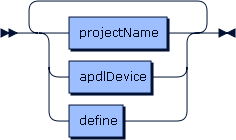
\includegraphics[scale=0.7]{img/ebnf_grammar/program}
\section*{projectName}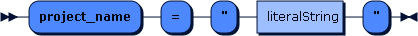
\includegraphics[scale=0.7]{img/ebnf_grammar/projectName}
\section*{apdlDevice}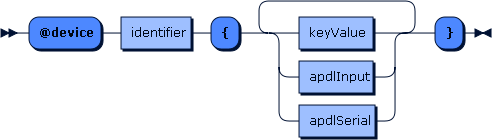
\includegraphics[scale=0.7]{img/ebnf_grammar/apdlDevice}
\section*{defines}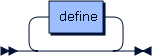
\includegraphics[scale=0.7]{img/ebnf_grammar/defines}
\section*{define}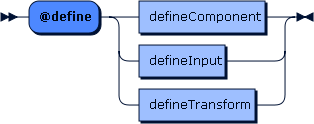
\includegraphics[scale=0.7]{img/ebnf_grammar/define}
\section*{defineComponent}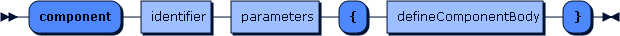
\includegraphics[scale=0.7]{img/ebnf_grammar/defineComponent}

\section*{apdlInput}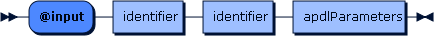
\includegraphics[scale=0.7]{img/ebnf_grammar/apdlInput}
\section*{apdlSerial}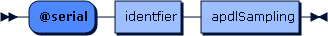
\includegraphics[scale=0.7]{img/ebnf_grammar/apdlSerial}
\section*{apdlParameters}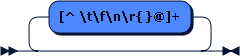
\includegraphics[scale=0.7]{img/ebnf_grammar/apdlParameters}
\section*{apdlSampling}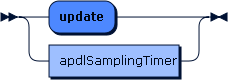
\includegraphics[scale=0.7]{img/ebnf_grammar/apdlSampling}
\section*{apdlSamplingTimer}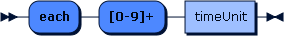
\includegraphics[scale=0.7]{img/ebnf_grammar/apdlSamplingTimer}
\section*{timeUnit}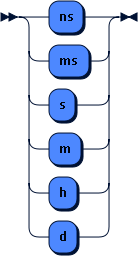
\includegraphics[scale=0.7]{img/ebnf_grammar/timeUnit}
\section*{type}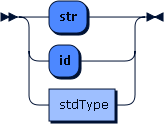
\includegraphics[scale=0.7]{img/ebnf_grammar/type}
\section*{stdType}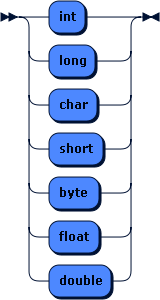
\includegraphics[scale=0.7]{img/ebnf_grammar/stdType}
\section*{arg}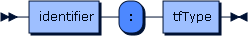
\includegraphics[scale=0.7]{img/ebnf_grammar/arg}

\section*{defineInput}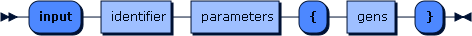
\includegraphics[scale=0.7]{img/ebnf_grammar/defineInput}
\section*{defineTransform}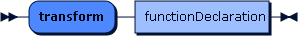
\includegraphics[scale=0.7]{img/ebnf_grammar/defineTransform}
\section*{defineComponentBody}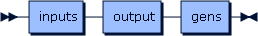
\includegraphics[scale=0.7]{img/ebnf_grammar/defineComponentBody}

\section*{parameters}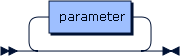
\includegraphics[scale=0.7]{img/ebnf_grammar/parameters}
\section*{parameter}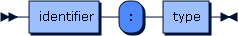
\includegraphics[scale=0.7]{img/ebnf_grammar/parameter}

\section*{inputs}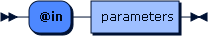
\includegraphics[scale=0.7]{img/ebnf_grammar/inputs}
\section*{output}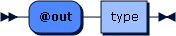
\includegraphics[scale=0.7]{img/ebnf_grammar/output}
\section*{gens}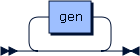
\includegraphics[scale=0.7]{img/ebnf_grammar/gens}
\section*{gen}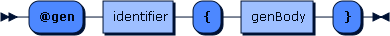
\includegraphics[scale=0.7]{img/ebnf_grammar/gen}
\section*{genBody}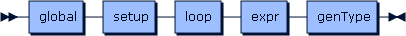
\includegraphics[scale=0.7]{img/ebnf_grammar/genBody}
\section*{global}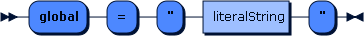
\includegraphics[scale=0.7]{img/ebnf_grammar/global}
\section*{setup}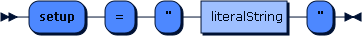
\includegraphics[scale=0.7]{img/ebnf_grammar/setup}
\section*{loop}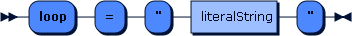
\includegraphics[scale=0.7]{img/ebnf_grammar/loop}
\section*{expr}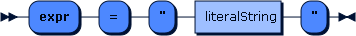
\includegraphics[scale=0.7]{img/ebnf_grammar/expr}
\section*{genType}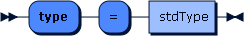
\includegraphics[scale=0.7]{img/ebnf_grammar/genType}
\section*{literalString}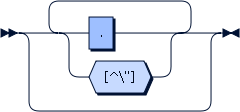
\includegraphics[scale=0.7]{img/ebnf_grammar/literalString}

\section*{returnType}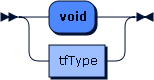
\includegraphics[scale=0.7]{img/ebnf_grammar/returnType}
\section*{tfType}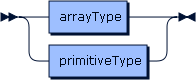
\includegraphics[scale=0.7]{img/ebnf_grammar/tfType}
\section*{primitiveType}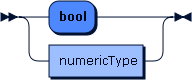
\includegraphics[scale=0.7]{img/ebnf_grammar/primitiveType}
\section*{numericType}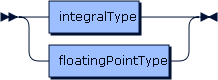
\includegraphics[scale=0.7]{img/ebnf_grammar/numericType}
\section*{arrayType}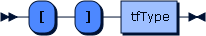
\includegraphics[scale=0.7]{img/ebnf_grammar/arrayType}
\section*{integralType}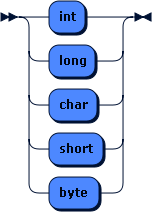
\includegraphics[scale=0.7]{img/ebnf_grammar/integralType}
\section*{floatingPointType}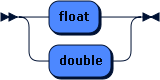
\includegraphics[scale=0.7]{img/ebnf_grammar/floatingPointType}

\section*{constantExpr}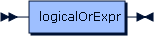
\includegraphics[scale=0.7]{img/ebnf_grammar/constantExpr}
\section*{logicalOrExpr}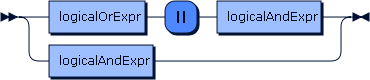
\includegraphics[scale=0.7]{img/ebnf_grammar/logicalOrExpr}
\section*{logicalAndExpr}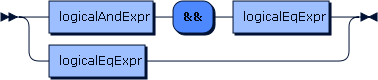
\includegraphics[scale=0.7]{img/ebnf_grammar/logicalAndExpr}
\section*{logicalEqExpr}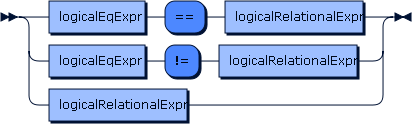
\includegraphics[scale=0.7]{img/ebnf_grammar/logicalEqExpr}
\section*{logicalRelationalExpr}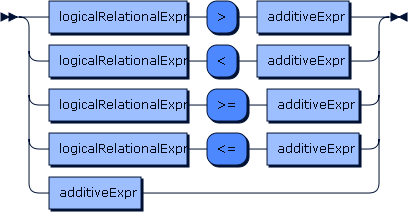
\includegraphics[scale=0.7]{img/ebnf_grammar/logicalRelationalExpr}
\section*{additiveExpr}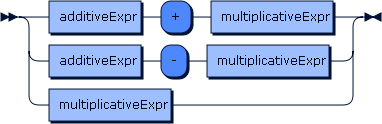
\includegraphics[scale=0.7]{img/ebnf_grammar/additiveExpr}
\section*{multiplicativeExpr}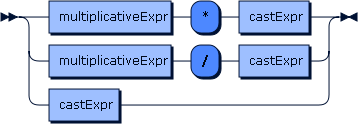
\includegraphics[scale=0.7]{img/ebnf_grammar/multiplicativeExpr}
\section*{castExpr}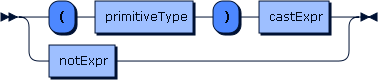
\includegraphics[scale=0.7]{img/ebnf_grammar/castExpr}
\section*{notExpr}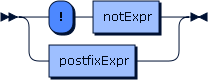
\includegraphics[scale=0.7]{img/ebnf_grammar/notExpr}
\section*{postfixExpr}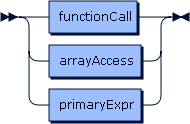
\includegraphics[scale=0.7]{img/ebnf_grammar/postfixExpr}
\section*{primaryExpr}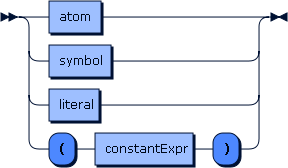
\includegraphics[scale=0.7]{img/ebnf_grammar/primaryExpr}
\section*{functionCall}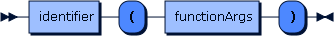
\includegraphics[scale=0.7]{img/ebnf_grammar/functionCall}
\section*{functionArgs}\includegraphics[scale=0.7]{img/ebnf_grammar/functionArgs}
\section*{arrayAccess}\includegraphics[scale=0.7]{img/ebnf_grammar/arrayAccess}
\section*{atom}\includegraphics[scale=0.7]{img/ebnf_grammar/atom}
\section*{symbol}\includegraphics[scale=0.7]{img/ebnf_grammar/symbol}
\section*{literal}\includegraphics[scale=0.7]{img/ebnf_grammar/literal}
\section*{assignExpr}\includegraphics[scale=0.7]{img/ebnf_grammar/assignExpr}
\section*{identifier}\includegraphics[scale=0.7]{img/ebnf_grammar/identifier}

\section*{functionDeclaration}\includegraphics[scale=0.7]{img/ebnf_grammar/functionDeclaration}
\section*{functionHeader}\includegraphics[scale=0.7]{img/ebnf_grammar/functionHeader}
\section*{functionBody}\includegraphics[scale=0.7]{img/ebnf_grammar/functionBody}
\section*{block}\includegraphics[scale=0.7]{img/ebnf_grammar/block}
\section*{statement}\includegraphics[scale=0.7]{img/ebnf_grammar/statement}
\section*{selectionStatement}\includegraphics[scale=0.7]{img/ebnf_grammar/selectionStatement}
\section*{loops}\includegraphics[scale=0.7]{img/ebnf_grammar/loops}
\section*{jump}\includegraphics[scale=0.7]{img/ebnf_grammar/jump}
\section*{exprStatement}\includegraphics[scale=0.7]{img/ebnf_grammar/exprStatement}

\section*{ifThenElse}\includegraphics[scale=0.7]{img/ebnf_grammar/ifThenElse}
\section*{ifThen}\includegraphics[scale=0.7]{img/ebnf_grammar/ifThen}
\section*{while}\includegraphics[scale=0.7]{img/ebnf_grammar/while}
\section*{doWhile}\includegraphics[scale=0.7]{img/ebnf_grammar/doWhile}

\section*{declaration}\includegraphics[scale=0.7]{img/ebnf_grammar/declaration}
\section*{newArray}\includegraphics[scale=0.7]{img/ebnf_grammar/newArray}
\section*{arrayInit}\includegraphics[scale=0.7]{img/ebnf_grammar/arrayInit}
\section*{newVal}\includegraphics[scale=0.7]{img/ebnf_grammar/newVal}
\section*{newVar}\includegraphics[scale=0.7]{img/ebnf_grammar/newVar}


\chapter{APDL Recursive Inclusion Algorithm Implementation in Scala}
\label{app:algo_recursive_construct}

\begin{scalacode}
def generateInputs(out: ApdlPrintWriter): Unit = {
  // Generate default input
  debug(s"\tGenerate default inputs")
  generateDefaultInputs(out)
  // Make the symbolTable for non-default input
  debug(s"\tGenerate non default inputs")
  generateNonDefaultInputs(out)
}

def generateNonDefaultInputs(out: ApdlPrintWriter): Unit = {
  val inputs = device.inputs
  val nonDefaultInputs = inputs.filter(isNonDefault)

  // For each inputs, take the ones who are generable
  def process(inputs: List[ApdlInput]): Unit = if (inputs.nonEmpty) {
    val (generableInputs, nonGenerableInputs) = inputs.partition(isGenerable)
    generableInputs.foreach { i =>
      if (isTransform(i)) {
        val sourceInput = symbolTable.get(i.args.head) match {
          case default: InputDefault => default
          case transformed: InputTransformed => transformed
          case componented: InputComponented => componented
          case _ => throw new ApdlProjectException(s"Can't find source input for input ${i.identifier}")
        }
        val definition = defines.find(_.identifier == i.defineInputIdentifier) match {
          case Some(value) => value
          case None => throw new ApdlProjectException(s"Unknow define for input ${i.identifier}")
        }
        assume(definition.isInstanceOf[ApdlDefineTransform])

        // code generation
        val functionDecl = definition.asInstanceOf[ApdlDefineTransform].functionDecl

        if (!symbolTable.contains(functionDecl.header.identifier)) {
          // A transform is a function
          out.printlnFunction {
            s"""
                | // Transform ${functionDecl.header.identifier}
                | ${transformCodeGen(functionDecl)}
                | // End transform ${functionDecl.header.identifier}
            """.stripMargin
          }
          // Add the transform into the symbol table
          symbolTable.add(functionDecl.header.identifier, Transform(functionDecl))
        }
        symbolTable.add(i.identifier, InputTransformed(i.identifier, definition.asInstanceOf[ApdlDefineTransform], sourceInput))

      } else if (isComponented(i)) {

        val definition = defines.find(_.identifier == i.defineInputIdentifier) match {
          case Some(value) => value
          case None => throw new ApdlProjectException(s"Unknow define for input ${i.identifier}")
        }

        assume(definition.isInstanceOf[ApdlDefineComponent])

        val component = definition.asInstanceOf[ApdlDefineComponent]

        val nbNonInputs = component.parameters.length
        val args = i.args.drop(nbNonInputs)
        val sourceInputs: List[Input] = symbolTable.gets(args).map {
          case default: InputDefault => default
          case transformed: InputTransformed => transformed
          case componented: InputComponented => componented
          case _ => throw new ApdlProjectException(s"Can't find source input for input ${i.identifier}")
        }


        symbolTable.add(i.identifier, InputComponented(i.identifier, definition.asInstanceOf[ApdlDefineComponent], sourceInputs))

      } else {
        // something is wrong...
        throw new ApdlProjectException(s"Input ${i.identifier} from device ${device.name} encountered some problems")
      }
    }
    process(nonGenerableInputs)
  }

  process(nonDefaultInputs)
}

def isTransform(input: ApdlInput): Boolean = defines.find {
  case ApdlDefineTransform(functionDecl) => functionDecl.header.identifier == input.defineInputIdentifier
  case _ => false
} match {
  case Some(value) =>
    assert(value.isInstanceOf[ApdlDefineTransform])
    assert(input.args.length == 1)
    true
  case None => false
}

def isComponented(input: ApdlInput): Boolean = defines.find {
  case component: ApdlDefineComponent => component.identifier == input.defineInputIdentifier
  case _ => false
} match {
  case Some(value) =>
    assert(value.isInstanceOf[ApdlDefineComponent])
    true
  case None => false
}

def isGenerable(input: ApdlInput): Boolean = {
  if (isTransform(input)) {
    assert(input.args.length == 1)
    val sourceInput = input.args.head
    symbolTable.contains(sourceInput)
  }
  else if (isComponented(input)) {
    val componentDefine = defines.find(_.identifier == input.defineInputIdentifier) match {
      case Some(value) => value match {
        case component: ApdlDefineComponent => component
        case _ => throw new ApdlProjectException(s"Unexpected definition found for input ${input.identifier} from device ${device.name}")
      }
      case None => throw new ApdlProjectException(s"Unknow define component for input ${input.identifier} from device ${device.name}")
    }
    val nbNonInputs = componentDefine.parameters.length
    val args = input.args.drop(nbNonInputs)
    args.forall(symbolTable.contains)
  }
  else {
    throw new ApdlProjectException(s"Wrong input type for input ${input.identifier} from device ${device.name}")
  }
}

def isNonDefault(input: ApdlInput): Boolean = {
  !isDefault(input)
}

def isDefault(input: ApdlInput): Boolean = {
  defines.find(_.identifier == input.defineInputIdentifier) match {
    case Some(definition) => definition match {
      case _: ApdlDefineInput => true
      case _: ApdlDefineComponent => false
      case _: ApdlDefineTransform => false
    }
    case None =>
      throw new ApdlProjectException(s"Unknow type for input ${input.identifier}")
  }
}

// Generate the default input inside the symbol table
def generateDefaultInputs(out: ApdlPrintWriter): Unit = device.inputs.foreach { input =>
  defines.find(_.identifier == input.defineInputIdentifier) match {
    case Some(definition) => definition match {
      case ApdlDefineInput(name, parameters, gens) =>
        // A default input

        val gen = gens.getOrElse(framework.identifier, throw new ApdlProjectException(s"Unknow framework $framework for input definition : $name"))

        implicit val args = zipArgWithIdentifier(input.args, parameters, List()) + ("id" -> IdGenerator.nextVariable(input.identifier))

        out.printlnGlobal(gen.global.replaceWithArgs)
        out.printlnSetup(gen.setup.replaceWithArgs)
        out.printlnLoop(gen.loop.replaceWithArgs)

        symbolTable.add(input.identifier, InputDefault(
          input.identifier,
          definition.asInstanceOf[ApdlDefineInput],
          input.args,
          gen.expr.replaceWithArgs))
      case _ =>
    }
    case None => throw new ApdlProjectException(s"Unknow type for input ${input.identifier}")
  }
}
\end{scalacode}

\chapter{Generators Implementation for Property-based Testing}
\label{app:generators_property_based_testing}

\section*{GeneratorUtils.scala}
\scalafile{../APDL/src/test/scala/GeneratorUtils.scala}

\chapter{APDL Code Generator for Property-based Testing}
\label{app:apdl_code_generator_for_test}

\section*{DslApdlBackendGenerators.scala}
\scalafile{../APDL/src/main/scala/apdl/parser/DslApdlBackendGenerators.scala}

\section*{TransformApdlBackendGenerators.scala}
\scalafile{../APDL/src/main/scala/apdl/parser/TransformApdlBackendGenerators.scala}

\chapter{Implementation of the Preprocessor's Tests}
\label{app:includes_tests}

\section*{IncludeTest.scala}
\scalafile{../APDL/src/test/scala/IncludeTest.scala}

\chapter{APDL Component file}
\label{app:apdl_component_apdl}

\section*{apdl\_component.apdl}
\begin{apdlcode}
@define input analogInput pin:str {
    @gen mbed {
        global = "AnalogIn @id(@pin);"
        setup = ""
        loop = ""
        expr = "@id.read()"
        type = float
    }
    @gen arduino {
        global = ""
        setup = ""
        loop = ""
        expr = "analogRead(@pin)"
        type = int
    }
}

@define input digitalInput pin:str {
    @gen mbed {
        global = "DigitalIn @id(Dpin);"
        setup = ""
        loop = ""
        expr = "@id.read()"
        type = float
    }
    @gen arduino {
        global = ""
        setup = ""
        loop = ""
        expr = "digitalRead(@pin)"
        type = int
    }
}
\end{apdlcode}

\end{appendices}
